\begin{quote}
	计算机系统中没有魔法. \hfill -- 蒋炎岩
\end{quote}



\section{数据与数据结构}

\ti{中学的练习题与计算机中的算法}

计算机的一个重要的功能是存储和操作数据. 那么从“数据”的角度看,通过算法希望计算机帮我们解的“题”与你们中学数学课上解的题有什么不同?

事实上, 算法的输入是满足特定条件的对象的集合(“问题空间”),算法必须能保证对该集合中“任一对象”均能计算出正确的结果。程序是算法的“实现”,其“每一次”执行处理的是某个特定数据对象(问题实例)。

因此,中学数学课中的那些“题目”是我们这里讨论的算法问题的“实例”。因为我们只需要对于单一的个体进行回答. 

对于算法而言, 为什么讨论计算机问题求解必须讨论“数据”?首先, 输入数据必须以某种形式“放入”计算机;输出结果必须以某种形式的数据呈现给用户;问题求解过程可以看作“数据转换”过程,这个过程如果有多个步骤组成,则每个步骤可能需要以中间形式暂时存放,供后面的步骤使用。

最基本的数据可以说为变量了. 在第一章中, 我们说明了我们认为变量是存储一个``东西''的盒子. 我们说这个``盒子''其实有两种形式. 按值(by value)或者按引用(by reference). 见图. 

% TODO. 补充by value和by reference的图

比如, 在“冒泡”排序算法中,核心操作是“交换序列中两个元素(不妨说是$x$,$y$),其实现过程可以表示如下(注意:需要使用一个临时辅助变量$z$):
$$
\begin{aligned}
z&\leftarrow x\\
x&\leftarrow y\\
y&\leftarrow z	
\end{aligned}
$$

在C语言中, 为什么对变量要指定“类型”?首先, 变量的类型表示了这些变量够执行什么样的“操作”(运算). 我们为什么要给变量起名字? 其实变量名的本质在于. 变(常)量名是计算机存储区地址的“抽象”. 编程时关注的“位置”与计算机内的物理地址无关.

在数据结构中, “结构”究竟是什么?实际上, 控制结构与数据结构是计算机算法的两个侧面,数据结构不仅仅是关乎数据“如何放”。

\begin{quote}
	While \blue{control structures} serve to tell the processor \blue{where it should be going}, \red{data structures}, and the operations upon them, organize the data items in ways that enable it to \red{do whatever it should do} when it gets there.
\end{quote}

比如, “全班同学排好队!”是什么意思?首先, 每人有了一个“位置”。然后, 其实这个“位置”是相对的。其实, 如果安排一种按照位置进行的“游戏”,“到了什么位置就知道该做什么”。

这样我们就知道了程序设计语言中的数组到底是什么. 数组就相当于抽象的逻辑结构是“顺序”结构. 在计算机中的“实现”就是同类型数据的“序列”。程序设计语言为你提供了定义特定数组的“设施”. 物理位置就可以不用管了. 

我们选取的数据结构与控制结构的对应(图\ref{figs:cflow}). 来看几个例子. 

\begin{figure}
	\centering
	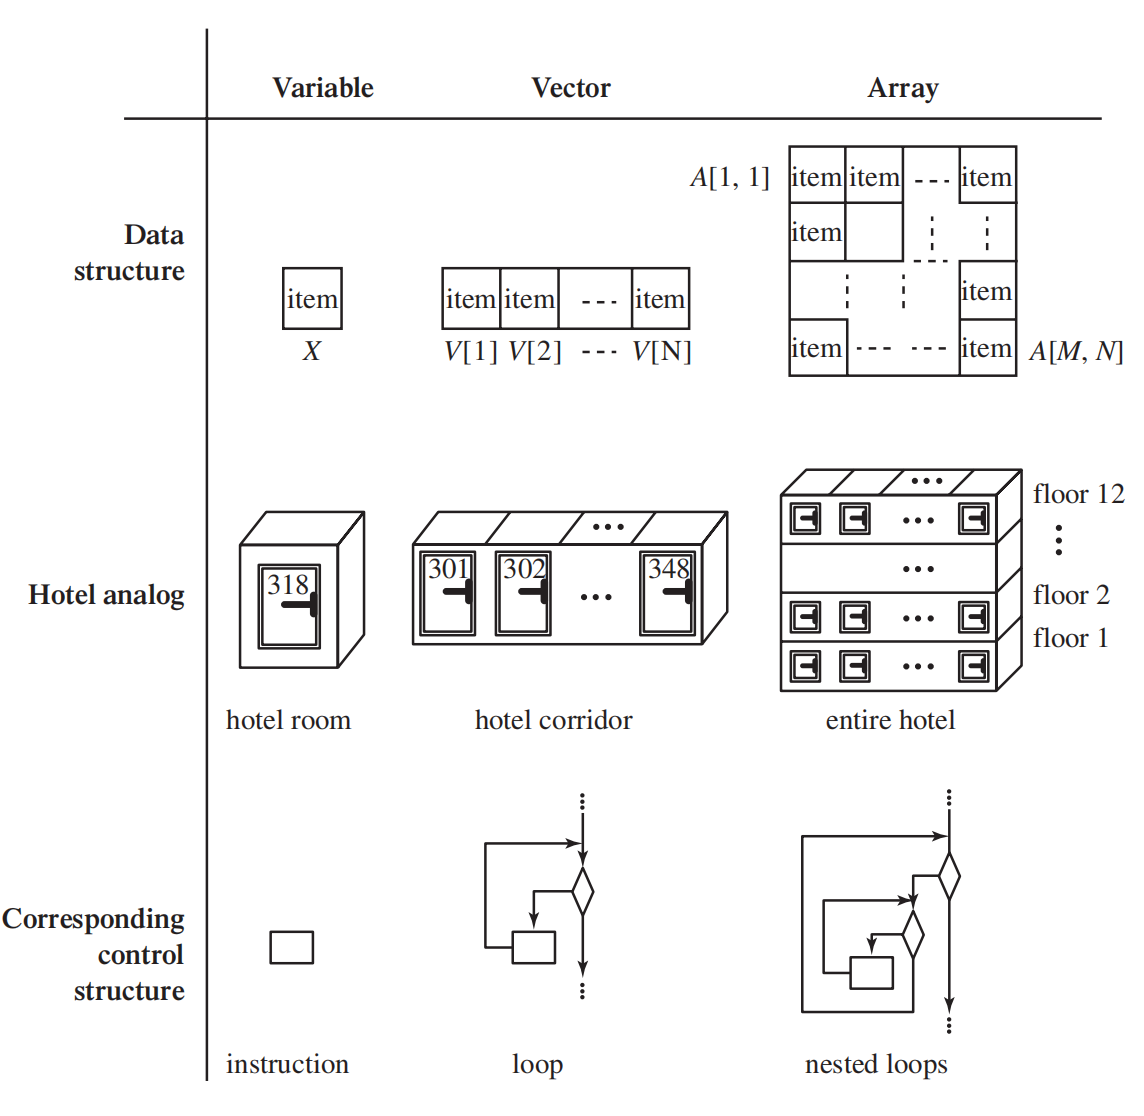
\includegraphics[scale=0.5]{4-programs/figs/structures}
	\caption{数据结构与控制结构的对应的例子}
	\label{figs:cflow}
	
\end{figure}

比如, 我们写了一个$n$维的数组, 但是可能想过, 数组维数的相对性. 比如一个二维数组可以写称为vector套vector. 

这就是数组的一些有趣的事情. 下面来总结一下. 数组结构的访问方式特点是什么,对于解题有什么好处?又带来什么不便?

数组元素使用“下标”确定其位置,而下标是顺序编排的,这对访问数组元素带来什么便利?正因为顺序编排,对于在应用中如果需要增删元素则必须“维护”相应的特性?

你若需要对数组元素进行如下操作,可能必须移动“整块”的其它元素:(1)在指定位置插入一个新元素;(2)删除某个位置上的元素但不留下“空挡”, 那么代价可能很大. 

数组实际上是通过连续编排下标将元素顺序连接成一个“结构”. 如果我们将“顺序连接”抽象为对用户“透明”的实现方式,那么数组就可以认为是“抽象数据类型”list的一种实现。list中“顺序”的概念是抽象的,可以用不同方式实现. 常用的linked-list可以认为是一种使用“指针”的实现。显然linked-list(链表)可以解决数组的不便。而且更适用于执行前无法确定序列长度的情况。

我们发现我们不关心这里面的数据到底是什么. 所谓“抽象数据类型”不涉及数据对象的性质以及其“存放”方式,仅通过操作定义体现在“解题”时的应用意义。比如, 简化的list由4个操作定义:(1)一个创建(插入)操作,两个“查询”操作,一个常量.

\begin{lstlisting}
list cons(obj newElement, oldList)
Precondition: none
Postcondition: if x=con(newElement, oldList)  then:
    (1) x refer to a newly created list
    (2) x!=nil
    (3) first(x)=newElement
    (4) rest(x)=oldList
obj first(list aList)
Precondition: aList!=nil

list rest(list aList)
Precondition: sList!=nil

list nil
\end{lstlisting}


\ti{抽象数据类型与问题求解}

我们来考察如下的两个情形: (1)在图书馆的书架某一层取一本书; (2) 在机场的饮水机旁取一个纸杯. 这两者有何不同?其实, 如果仅仅从“放置”的角度看,两者涉及的物体放置方式是一样的:“一个挨着一个的顺序结构”,不同的是对元素的操作方式。我们的操作方式是被受到限制的. 即使一样的“受限”操作方式,也可以有不同的“限”法:比如栈(stack)和队列(queue)在不同的问题的求解有不同的明显的意义。


比如判定输入字符串是否“回文(palindrome)”也就是从头读到尾与从尾读到头完全一样. 一个最朴素的想法就是通过数组的方式存储每一个字符, 然后正着倒着循环并且判断即可. 另一个例子是模拟一个排队的场景: 设想一个单服务柜台的运行状态,设定模拟总时间长度,随机生成“新顾客到达时间及其需要的服务处理时长”模拟可能的排队等待队列人数变化情况。假设服务能力与预期顾客需求量总量平衡。既然是``队列'', 我们就不允许新元素``插队''了. 

想一想大学里面选修课程的依赖, 以及家谱(family tree), 它们一般构成一个树的关系--这样非线性的内容是如何存在计算机中的呢? 事实上, 我们并不是真正的在内存里按照图形的样子进行存储的. 我们是使用引用的方式来把这个关系搞清楚的. 树的一个比较明显的特征是可分“层”. 

我们在内存里面是如何存储树的呢? 事实上, 我们只要在每个节点上打上它儿子节点的编号就行了. 这样我们在找子树的时候就可以按照编号去对应的位置去寻找了. 当然这只是一种方法, 其他的方法大同小异, 不过这样一个对应关系还是绕不过去的. 

\begin{figure}[htbp!]
	\centering
	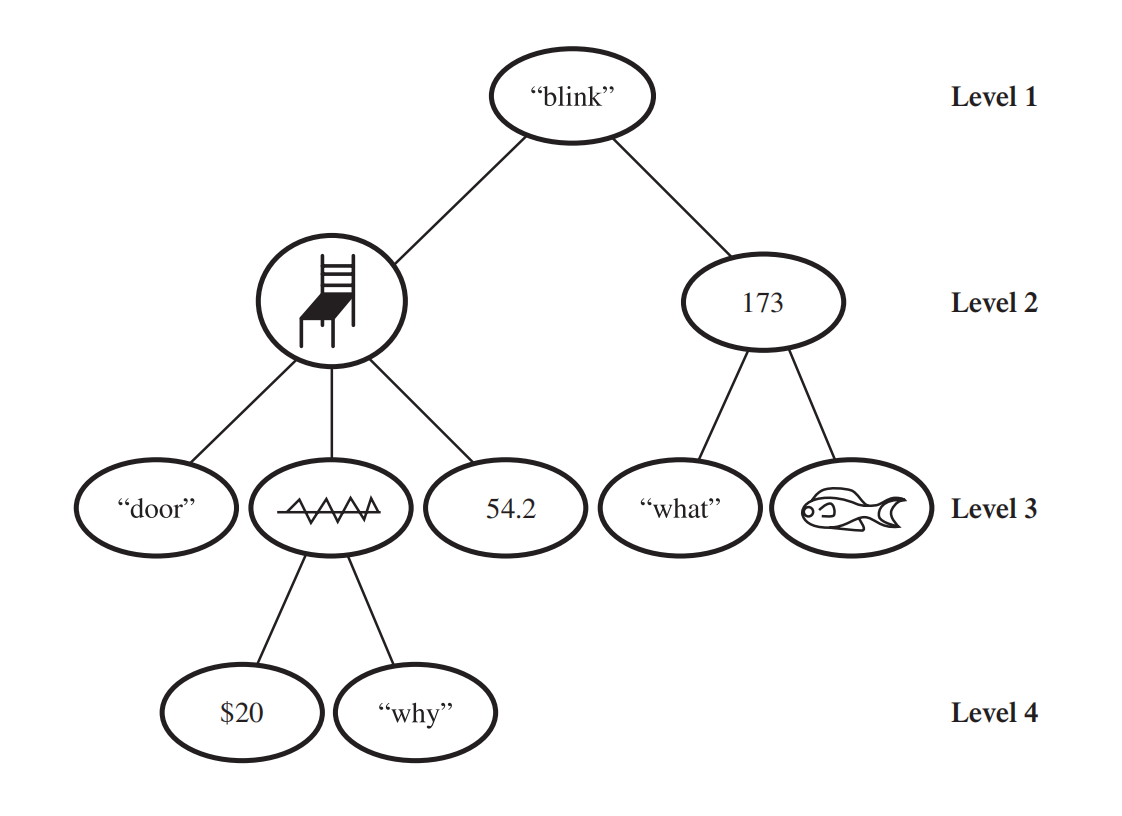
\includegraphics[scale=0.5]{4-programs/figs/tree}
	\caption{一棵``树''}
	\label{figs:tree-fig}
	
\end{figure}

如果这里是一个数组或者嵌套的数组, 我们可以很容易的看到它里面的所有的元素是什么. 那么如果是树我们应该如何看到它的内容呢? 

这就要回到我们如何看树了. 从非递归的视角来看, 我们有一个“结点”的集合$\set{A,B,\cdots,K}$, 以及一个“独特”的结点 – “根”:$A$. 根只有“出边”,没有“入边”. 其它任何结点有恰好一个“入边”, 这也就保证了每一个节点具有唯一的通路.  从递归视角来看, 会发现它有一个唯一的“根”结点. 假设根结点有$k$条出边,其另一端点为 $v_1,v_2,\cdots,v_k$,它们分别是$k$个无结点相交的树的根,这些树称为“子树”. 

从递归的视角来看树可以由很多的好处. 比如, 这就可以让我们发现如果要遍历一棵树, 那么先遍历左边子树, 在遍历右边的子树就行了. 这看上去比较抽象, 我们下面说几个比较有趣的例子. 

\textbf{例子1. 利用树排序. }(见图\ref{figs:tree-sort}) 首先, 将数组表示为“二分搜索树”. ``二分搜索树''的生成方式是这样的: 每个节点的左边节点的数值一定比它的值小, 右边的一定比它的值大. 以“深度优先”方式遍历树, 那么输出方式一定是从小到大的. 


\begin{figure}[htbp!]
	\centering
	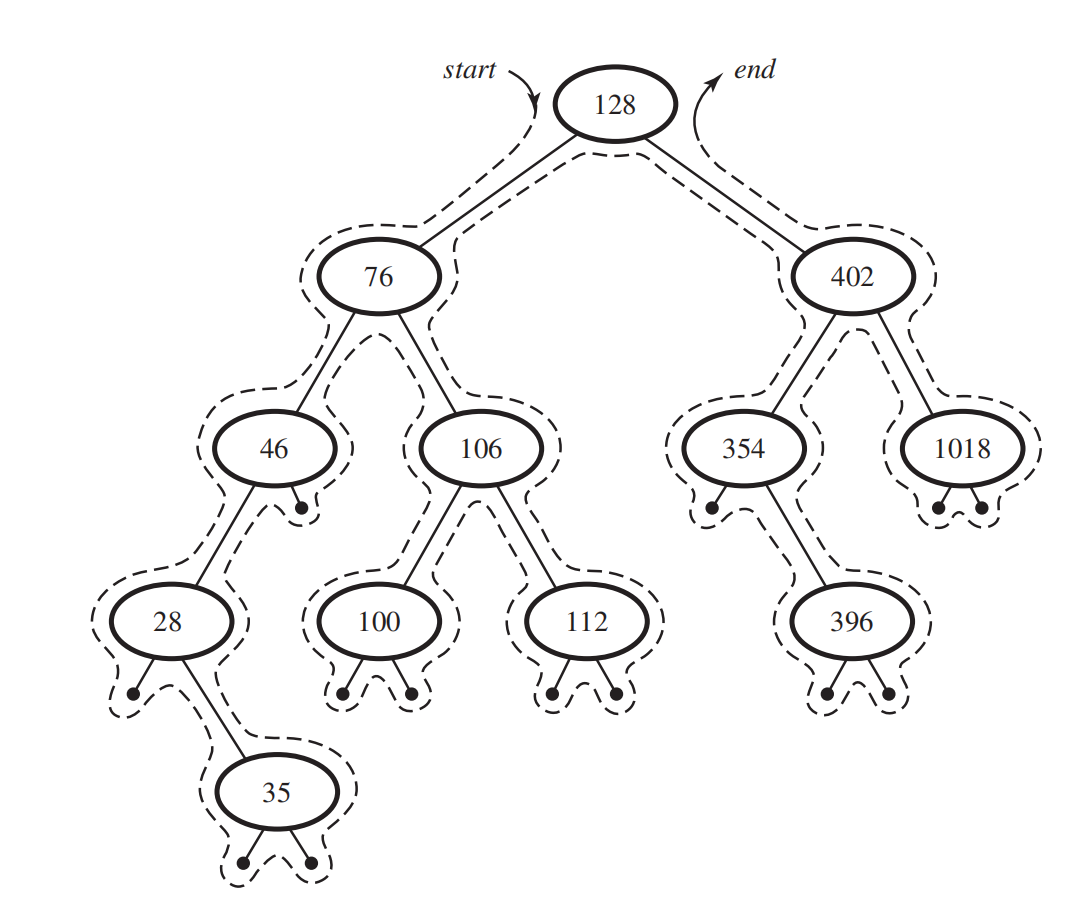
\includegraphics[scale=0.8]{4-programs/figs/tree-sort.png}
	\caption{用于排序的树}
	\label{figs:tree-sort}
	
\end{figure}

\textbf{例子2. 树结构和算数表达求值. }(见图\ref{figs:tree-eval}) 如算术表达式:$(10 + (( 22 – 3 \times 4) / 2 – 2 \times 2 ) \times (( 14 – 2) / (1 + 3 ) )$. 对应的表达式树就是这样的: 

\begin{figure}[htbp!]
	\centering
	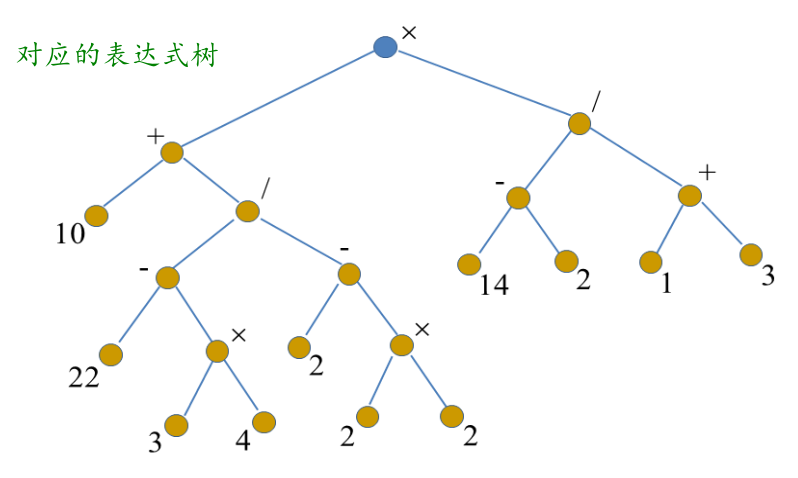
\includegraphics[scale=0.8]{4-programs/figs/exptree}
	\caption{由于表达式求值的树}
	\label{figs:tree-eval}
	
\end{figure}


我们使用Left-first traversal(Third-visit output, 称为“后序”). 

其实还有一个新的方法: 假如数字输出到一个堆栈中,每当遇到运算符则处理前面两个数,结果仍然是对的. 


\section{把算法告诉计算机}

我们可能会说, 把算法告诉计算机有什么难的? 写点代码就行了啊! 但计算机的最底层是01的组合, 我们今天并没有用0,1表述我们的算法. 

事实上, “早期”的程序员真的用0, 1编程序. 他们使用的是打孔纸带和操作系统进行. 其一般有三个部分组成. 如图. “指令”对应于“预制”的“微程序”(电路)的入口。计算机“能接受”这样的语言表述,但并不知道你究竟“想干什么”. 因为“编程自动化”远比“算法设计自动化”要容易! 

我们的计算机科学家
















